%%%%%%%%%%%%%%%%%%%%%%%%%%%%%%%%%%%%%%%%%
% Beamer Presentation
% LaTeX Template
% Version 1.0 (10/11/12)
%
% This template has been downloaded from:
% http://www.LaTeXTemplates.com
%
% License:
% CC BY-NC-SA 3.0 (http://creativecommons.org/licenses/by-nc-sa/3.0/)
%
%%%%%%%%%%%%%%%%%%%%%%%%%%%%%%%%%%%%%%%%%

%----------------------------------------------------------------------------------------
%	PACKAGES AND THEMES
%----------------------------------------------------------------------------------------

\documentclass{beamer}

\mode<presentation> {

% The Beamer class comes with a number of default slide themes
% which change the colors and layouts of slides. Below this is a list
% of all the themes, uncomment each in turn to see what they look like.

%\usetheme{default}
%\usetheme{AnnArbor}
%\usetheme{Antibes}
%\usetheme{Bergen}
%\usetheme{Berkeley}
%\usetheme{Berlin}
%\usetheme{Boadilla}
%\usetheme{CambridgeUS}
%\usetheme{Copenhagen}
%\usetheme{Darmstadt}
%\usetheme{Dresden}
%\usetheme{Frankfurt}
%\usetheme{Goettingen}
%\usetheme{Hannover}
%\usetheme{Ilmenau}
%\usetheme{JuanLesPins}
%\usetheme{Luebeck}
%\usetheme{Madrid}
%\usetheme{Malmoe}
%\usetheme{Marburg}
%\usetheme{Montpellier}
%\usetheme{PaloAlto}
\usetheme{Pittsburgh}
%\usetheme{Rochester}
%\usetheme{Singapore}
%\usetheme{Szeged}
%\usetheme{Warsaw}

% As well as themes, the Beamer class has a number of color themes
% for any slide theme. Uncomment each of these in turn to see how it
% changes the colors of your current slide theme.

%\usecolortheme{albatross}
\usecolortheme{beaver}
%\usecolortheme{beetle}
%\usecolortheme{crane}
%\usecolortheme{dolphin}
%\usecolortheme{dove}
%\usecolortheme{fly}
%\usecolortheme{lily}
%\usecolortheme{orchid}
%\usecolortheme{rose}
%\usecolortheme{seagull}
%\usecolortheme{seahorse}
%\usecolortheme{whale}
%\usecolortheme{wolverine}

%\setbeamertemplate{footline} % To remove the footer line in all slides uncomment this line
%\setbeamertemplate{footline}[page number] % To replace the footer line in all slides with a simple slide count uncomment this line

%\setbeamertemplate{navigation symbols}{} % To remove the navigation symbols from the bottom of all slides uncomment this line
}

\usepackage{graphicx} % Allows including images
\usepackage{booktabs} % Allows the use of \toprule, \midrule and \bottomrule in tables

\usepackage{fontspec}
\setsansfont{Calibri}[
    Path=Font/,
    Scale=0.9,
    Extension = .ttf,
    UprightFont=*-Regular,
    BoldFont=*-Bold,
    ItalicFont=*-Italic,
    BoldItalicFont=*-BoldItalic
    ]
\usepackage{unicode-math}
\setmathfont{Libertinus Math}% 使用默认的数学字体或你偏好的数学字体 Latin Modern Math/Libertinus Math

\usepackage{ragged2e}
\justifying\let\raggedright\justifying %两端对齐

 \usepackage{tcolorbox} 
%----------------------------------------------------------------------------------------
%	TITLE PAGE
%----------------------------------------------------------------------------------------

\title[Asset Pricing]{\textbf{Asset Pricing}} % The short title appears at the bottom of every slide, the full title is only on the title page

\subtitle{9. ICAPM Other Version}

\author[Cheng Hang]{Cheng Hang} % Your name
\institute[DUFE] % Your institution as it will appear on the bottom of every slide, may be shorthand to save space
{School of Fintech \\
Dongbei University of Finance \& Economics \\ % Your institution for the title page
\medskip
\textbf{chenghangch@qq.com}% Your email address
}
\date{\today} % Date, can be changed to a custom date

	\AtBeginSection[]
{
	\begin{frame}{Content}
		\tableofcontents[sectionstyle=show/shaded,subsectionstyle=show/shaded/hide] %这几个参数我也不知道该如何准确地解释，反正它们最终的效果是突出显示当前章节，而其它章节都进行了淡化处理
		\addtocounter{framenumber}{-1}  %目录页不计算页码
	\end{frame}
}

%----------------------------------------------------------------------------------------
%	Begin
%----------------------------------------------------------------------------------------

\begin{document}

\begin{frame}
\titlepage % Print the title page as the first slide
\end{frame}


\section{Wealth Version}

\begin{frame}[allowframebreaks]
    \frametitle{From Continuation Utility to Wealth Return: Motivation}
    
    \textbf{The problem with the baseline SDF:}
    \begin{equation*}
        M_{t+1} = \delta \left( \frac{C_{t+1}}{C_t} \right)^{-1/\psi} \left( \frac{V_{t+1}}{\mu_t(V_{t+1})} \right)^{-(\gamma-1/\psi)}
    \end{equation*}
    
    \textbf{Challenge:} Continuation utility $V_{t+1}$ is not observable!
    \begin{itemize}
        \item $V_{t+1}$ represents lifetime utility from period $t+1$ onward
        \item Depends on entire future consumption path
        \item Cannot be directly measured in data
    \end{itemize}
    
    \textbf{Goal:} Express the SDF in terms of observable quantities:
    \begin{itemize}
        \item Consumption growth: $C_{t+1}/C_t$ (observable)
        \item Return on wealth portfolio: $R_{W,t+1}$ (observable or can be proxied)
    \end{itemize}
    
    \framebreak
    
    \textbf{Key insight:} Use the intertemporal budget constraint to link continuation utility to wealth and consumption.
    
    \textbf{Budget constraint:}
    \begin{equation*}
        W_{t+1} = (W_t - C_t)(1 + R_{W,t+1})
    \end{equation*}
    
    where:
    \begin{itemize}
        \item $W_t$: financial wealth at time $t$
        \item $C_t$: consumption at time $t$
        \item $W_t - C_t$: savings (invested in the wealth portfolio)
        \item $R_{W,t+1}$: return on the wealth portfolio from $t$ to $t+1$
    \end{itemize}
    
    \textbf{Economic interpretation:} The wealth portfolio is the market portfolio of all investable assets. In equilibrium, the representative agent holds this portfolio.
\end{frame}

\begin{frame}[allowframebreaks]
    \frametitle{Step 1: Value Function Conjecture}
    
    \textbf{Key conjecture:} The value function is linear in wealth:
    \begin{equation*}
        V_t = \phi(X_t) W_t
    \end{equation*}
    
    where $X_t$ represents state variables (e.g., expected growth rate, volatility).
    
    \textbf{Why is this conjecture reasonable?}
    \begin{itemize}
        \item Both the time aggregator $f(C, v)$ and certainty equivalent $\mu(\cdot)$ are homogeneous of degree 1
        \item If you double both consumption and continuation utility, value doubles
        \item This implies value should be proportional to the scale variable (wealth)
    \end{itemize}
    
    \framebreak
    
    \textbf{Implication for consumption policy:}
    
    If $V_t = \phi(X_t) W_t$, then optimal consumption is a constant fraction of wealth:
    \begin{equation*}
        C_t = \psi_t W_t
    \end{equation*}
    
    where $\psi_t \equiv C_t/W_t$ is the consumption-wealth ratio (depends on state $X_t$).
    
    \textbf{This gives us:}
    \begin{equation*}
        \phi_t = (1-\delta)^{1/\rho} \psi_t^{(\rho-1)/\rho}
    \end{equation*}
    
    where $\rho \equiv 1 - 1/\psi$ (we will verify this shortly).
\end{frame}

\begin{frame}[allowframebreaks]
    \frametitle{Step 2: Rewrite the Recursive Utility}
    
    \textbf{Starting from:}
    \begin{equation*}
        V_t = \left[ (1-\delta)C_t^{\rho} + \delta \mu_t(V_{t+1})^{\rho} \right]^{1/\rho}
    \end{equation*}
    
    where $\rho = 1 - 1/\psi$ and $\mu_t(V_{t+1}) = \left[ E_t[V_{t+1}^{1-\gamma}] \right]^{1/(1-\gamma)}$.
    
    \textbf{Substitute $V_{t+1} = \phi_{t+1} W_{t+1}$:}
    \begin{equation*}
        \mu_t(V_{t+1}) = \left[ E_t[(\phi_{t+1} W_{t+1})^{1-\gamma}] \right]^{1/(1-\gamma)}
    \end{equation*}
    
    Let $\alpha \equiv 1 - \gamma$. Then:
    \begin{equation*}
        \mu_t(V_{t+1}) = \left[ E_t[\phi_{t+1}^{\alpha} W_{t+1}^{\alpha}] \right]^{1/\alpha}
    \end{equation*}
    
    \framebreak
    
    \textbf{Use the budget constraint $W_{t+1} = (W_t - C_t)(1 + R_{W,t+1})$:}
    \begin{equation*}
        \mu_t(V_{t+1}) = \left[ E_t[\phi_{t+1}^{\alpha} ((W_t - C_t)(1 + R_{W,t+1}))^{\alpha}] \right]^{1/\alpha}
    \end{equation*}
    
    Factor out $(W_t - C_t)^{\alpha}$:
    \begin{equation*}
        \mu_t(V_{t+1}) = (W_t - C_t) \left[ E_t[\phi_{t+1}^{\alpha} (1 + R_{W,t+1})^{\alpha}] \right]^{1/\alpha}
    \end{equation*}
    
    \framebreak
    
    \textbf{Define:}
    \begin{equation*}
        \mu_t^* \equiv \left[ E_t[\phi_{t+1}^{\alpha} (1 + R_{W,t+1})^{\alpha}] \right]^{1/\alpha}
    \end{equation*}
    
    This is known at time $t$ and captures the expected return on the wealth portfolio adjusted for risk.
    
    \textbf{Then:}
    \begin{equation*}
        \mu_t(V_{t+1}) = (W_t - C_t) \mu_t^*
    \end{equation*}
    
    \framebreak
    
    \textbf{Substitute back into the value function:}
    \begin{equation*}
        V_t = \left[ (1-\delta)C_t^{\rho} + \delta [(W_t - C_t) \mu_t^*]^{\rho} \right]^{1/\rho}
    \end{equation*}
    
    Factor out $W_t$:
    \begin{equation*}
        V_t = W_t \left[ (1-\delta)\left(\frac{C_t}{W_t}\right)^{\rho} + \delta \left(1 - \frac{C_t}{W_t}\right)^{\rho} (\mu_t^*)^{\rho} \right]^{1/\rho}
    \end{equation*}
    
    Using $\psi_t = C_t/W_t$:
    \begin{equation*}
        V_t = W_t \left[ (1-\delta)\psi_t^{\rho} + \delta (1 - \psi_t)^{\rho} (\mu_t^*)^{\rho} \right]^{1/\rho}
    \end{equation*}
    
    \textbf{This confirms our conjecture: $V_t = \phi_t W_t$ where $\phi_t$ is the term in brackets.}
\end{frame}

\begin{frame}[allowframebreaks]
    \frametitle{Step 3: First-Order Condition for Consumption}
    
    \textbf{The agent's problem at time $t$:}
    \begin{equation*}
        \max_{C_t} V_t = \left[ (1-\delta)C_t^{\rho} + \delta [(W_t - C_t) \mu_t^*]^{\rho} \right]^{1/\rho}
    \end{equation*}
    
    \textbf{FOC with respect to $C_t$:}
    \begin{equation*}
        (1-\delta) \rho C_t^{\rho-1} = \delta \rho (W_t - C_t)^{\rho-1} (\mu_t^*)^{\rho}
    \end{equation*}
    
    Simplify ($\rho$ cancels):
    \begin{equation*}
        (1-\delta) C_t^{\rho-1} = \delta (W_t - C_t)^{\rho-1} (\mu_t^*)^{\rho}
    \end{equation*}
    
    \framebreak
    
    \textbf{Rearrange:}
    \begin{equation*}
        \frac{(1-\delta)}{\delta} = \frac{(W_t - C_t)^{\rho-1}}{C_t^{\rho-1}} (\mu_t^*)^{\rho}
    \end{equation*}
    
    \begin{equation*}
        \frac{(1-\delta)}{\delta} = \left(\frac{W_t - C_t}{C_t}\right)^{\rho-1} (\mu_t^*)^{\rho}
    \end{equation*}
    
    Using $\psi_t = C_t/W_t$, we have $\frac{W_t - C_t}{C_t} = \frac{1-\psi_t}{\psi_t}$:
    \begin{equation*}
        \frac{(1-\delta)}{\delta} = \left(\frac{1-\psi_t}{\psi_t}\right)^{\rho-1} (\mu_t^*)^{\rho}
    \end{equation*}
    
    \framebreak
    
    \textbf{Solving for $(\mu_t^*)^{\rho}$:}
    \begin{equation*}
        (\mu_t^*)^{\rho} = \frac{(1-\delta)}{\delta} \left(\frac{\psi_t}{1-\psi_t}\right)^{\rho-1}
    \end{equation*}
    
    \textbf{Recall the definition:}
    \begin{equation*}
        \mu_t^* = \left[ E_t[\phi_{t+1}^{\alpha} (1 + R_{W,t+1})^{\alpha}] \right]^{1/\alpha}
    \end{equation*}
    
    where $\alpha = 1 - \gamma$.
\end{frame}

\begin{frame}[allowframebreaks]
    \frametitle{Step 4: Derive the SDF from the Baseline Form}
    
    \textbf{Recall the baseline SDF:}
    \begin{equation*}
        M_{t+1} = \delta \left( \frac{C_{t+1}}{C_t} \right)^{-1/\psi} \left( \frac{V_{t+1}}{\mu_t(V_{t+1})} \right)^{-(\gamma-1/\psi)}
    \end{equation*}
    
    \textbf{Substitute $V_{t+1} = \phi_{t+1} W_{t+1}$ and $\mu_t(V_{t+1}) = (W_t - C_t)\mu_t^*$:}
    \begin{equation*}
        M_{t+1} = \delta \left( \frac{C_{t+1}}{C_t} \right)^{-1/\psi} \left( \frac{\phi_{t+1} W_{t+1}}{(W_t - C_t)\mu_t^*} \right)^{-(\gamma-1/\psi)}
    \end{equation*}
    
    \framebreak
    
    \textbf{Use the budget constraint $W_{t+1} = (W_t - C_t)(1 + R_{W,t+1})$:}
    \begin{equation*}
        M_{t+1} = \delta \left( \frac{C_{t+1}}{C_t} \right)^{-1/\psi} \left( \frac{\phi_{t+1} (1 + R_{W,t+1})}{\mu_t^*} \right)^{-(\gamma-1/\psi)}
    \end{equation*}
    
    Separate the terms:
    \begin{equation*}
        M_{t+1} = \delta \left( \frac{C_{t+1}}{C_t} \right)^{-1/\psi} \left(\frac{\phi_{t+1}}{\mu_t^*}\right)^{-(\gamma-1/\psi)} (1 + R_{W,t+1})^{-(\gamma-1/\psi)}
    \end{equation*}
    
    \framebreak
    
    \textbf{Key observation from the FOC:}
    
    From the first-order condition for consumption, we can show that:
    \begin{equation*}
        \phi_t = (1-\delta)^{1/\rho} \psi_t^{(\rho-1)/\rho}
    \end{equation*}
    
    This relationship, combined with the Euler equation, implies:
    \begin{equation*}
        E_t\left[\left(\frac{\phi_{t+1}}{\mu_t^*}\right)^{-\rho(\gamma-1/\psi)} (1 + R_{W,t+1})^{-\rho(\gamma-1/\psi)}\right] = \delta^{-\rho}(1-\delta)^{-1}
    \end{equation*}
    
    \framebreak
    
    \textbf{Through careful algebraic manipulation:}
    
    Define $\theta \equiv \frac{1-\gamma}{1-1/\psi}$. Then:
    \begin{itemize}
        \item $\gamma - 1/\psi = -(1-\gamma) + (1-1/\psi) = -(1-\gamma) + (1-1/\psi)$
        \item $\frac{\gamma - 1/\psi}{1-1/\psi} = \frac{-(1-\gamma) + (1-1/\psi)}{1-1/\psi} = 1 - \theta$
        \item Therefore: $\gamma - 1/\psi = (1-\theta)(1-1/\psi)$
    \end{itemize}
    
    \textbf{The composite preference parameter $\theta$ captures the combined effect of risk aversion and intertemporal substitution.}
\end{frame}

\begin{frame}[allowframebreaks]
    \frametitle{Step 5: The Wealth Return SDF}
    
    \textbf{After substituting the relationship between $\phi_{t+1}$ and model parameters:}
    
    \begin{tcolorbox}[colback=blue!5!white, colframe=blue!75!black, title=Wealth Return Form of Epstein-Zin SDF]
    \begin{equation*}
        M_{t+1} = \delta^{\theta} \left( \frac{C_{t+1}}{C_t} \right)^{-\theta/\psi} (1 + R_{W,t+1})^{-(1-\theta)}
    \end{equation*}
    \end{tcolorbox}
    
    where $\theta \equiv \frac{1-\gamma}{1-1/\psi}$ is the composite preference parameter. \\

    \textbf{Decomposition:}
    \begin{itemize}
        \item $\left[\delta \left( \frac{C_{t+1}}{C_t} \right)^{-1/\psi}\right]^{\theta}$: Intertemporal substitution component (raised to power $\theta$)
        \item $(1 + R_{W,t+1})^{-(1-\theta)}$: Return component (risk aversion effect through $1-\theta$)
    \end{itemize}
    
    \framebreak
    
    \textbf{Understanding the $\delta^{\theta}$ term:}
    
    \begin{itemize}
        \item The $\delta^{\theta}$ (not just $\delta$) arises from the homogeneity property of the value function
        \item When $\gamma = 1/\psi$ (i.e., $\theta = 1$), we get $\delta^{\theta} = \delta$ and the formula reduces to the power utility case
        \item The $\theta$ exponent reflects how the time discount factor is adjusted by the separation between risk aversion and intertemporal substitution
    \end{itemize}
    
    
    \framebreak
    
    \textbf{Log-linearized form:}
    
    Taking logs:
    \begin{equation*}
        m_{t+1} = \theta \log \delta - \frac{\theta}{\psi} \Delta c_{t+1} - (1-\theta) r_{w,t+1}
    \end{equation*}
    
    \textbf{SDF innovation (unexpected component):}
    \begin{tcolorbox}[colback=green!5!white, colframe=green!75!black, title=SDF Innovation (Wealth Return Form)]
    \begin{equation}
        \tilde{m}_{t+1} = -\frac{\theta}{\psi} \tilde{c}_{t+1} - (1-\theta) \tilde{r}_{w,t+1}\label{消费、财富形式的SDF}
    \end{equation}
    \end{tcolorbox}
    
    where lowercase letters denote logs and tilde denotes innovations.
    
\end{frame}


\begin{frame}[allowframebreaks]
    \frametitle{Economic Interpretation}
    
    \textbf{The SDF has two components:}
    \begin{equation*}
        \tilde{m}_{t+1} = -\frac{\theta}{\psi} \tilde{c}_{t+1} - (1-\theta) \tilde{r}_{w,t+1}
    \end{equation*}

    \textbf{Special cases:}
    
    \textbf{Case 1: Standard CRRA ($\gamma = 1/\psi$)}
    \begin{itemize}
        \item $\theta = 1$
        \item $\tilde{m}_{t+1} = -\gamma\tilde{c}_{t+1}$
        \item Only consumption growth matters (consumption CAPM)
    \end{itemize}
    
    \textbf{Case 2: Log utility ($\gamma = 1$)}
    \begin{itemize}
        \item $\theta = 0$
        \item $\tilde{m}_{t+1} = -\tilde{r}_{w,t+1}$
        \item Only wealth return matters (like traditional CAPM)
    \end{itemize}
    
    \framebreak
    
    \textbf{Case 3: General Epstein-Zin ($\gamma \neq 1/\psi$)}
    \begin{itemize}
        \item Both terms present with weights $\theta$ and $1-\theta$
        \item Nests both consumption CAPM and traditional CAPM
        \item When $\gamma > 1/\psi$ (empirically plausible):
        \begin{itemize}
            \item $0 < \theta < 1$
            \item Both consumption and wealth returns are priced
            \item Greater weight on wealth returns
        \end{itemize}
    \end{itemize}
 \end{frame}

\begin{frame}{Risk premium formula}
    
    Under lognormality:
    \begin{tcolorbox}[colback=red!5!white, colframe=red!75!black]
        \begin{equation*}
        E_t[r_{i,t+1}] - r_{f,t} = \frac{\theta}{\psi} \text{Cov}_t(r_{i,t+1}, \tilde{c}_{t+1}) + (1-\theta) \text{Cov}_t(r_{i,t+1}, \tilde{r}_{w,t+1})
    \end{equation*}
    \end{tcolorbox}
    
 
    \textbf{Interpretation:}
    \begin{itemize}
        \item Assets are priced based on two sources of systematic risk
        \item Consumption risk (short-run)
        \item Wealth return risk (captures both short-run and long-run components)
        \item The weights $\theta/\psi$ and $1-\theta$ depend on both $\gamma$ and $\psi$
    \end{itemize}
\end{frame}


\begin{frame}
    \frametitle{Risk-Free Rate}
    
    Under joint lognormality and homoskedasticity, the risk-free rate is:
    \begin{tcolorbox}[colback=blue!5!white, colframe=blue!75!black]
    \begin{equation*}
        % r_{f,t} = -\log(\delta) + \frac{1}{\psi} E_t[\Delta c_{t+1}] - \frac{1}{2} \frac{\theta}{\psi^2} \sigma_c^2 + \frac{\theta-1}{2} \sigma_w^2
        r_{f, t} \approx \underbrace{-\log \delta}_{\text {time preference }}+\underbrace{\frac{1}{\psi} E_t\left[\Delta c_{t+1}\right]}_{\text {Interperiod Substitution}}-\underbrace{- \frac{1}{2} \frac{\theta}{\psi^2} \sigma_c^2 + \frac{\theta-1}{2} \sigma_w^2}_{\text{ Precautionary Saving}}
    \end{equation*}
    \end{tcolorbox}
    
    \textbf{Key insight:} For given $\psi$, there is no quadratic term in $\gamma$
    
    \textbf{Why this matters:}
    \begin{itemize}
        \item Under CRRA, high $\gamma$ implies both high equity premium and counterfactually high risk-free rate
        
        \item With Epstein-Zin, we can increase $\gamma$ (to match equity premium) while keeping $\psi$ moderate
        
        \item This avoids the risk-free rate puzzle
    \end{itemize}
\end{frame}

\section{\textcolor{blue}{Campbell (1993)}: Without Consumption}

\begin{frame}
    \frametitle{Campbell (1993): Motivation}
    
    \textbf{The consumption data problem:}
    \begin{itemize}
        \item Aggregate consumption data is often measured with error
        \item Low frequency (quarterly or annual)
        \item Doesn't match timing of asset returns (daily, monthly)
        \item Consumption of stockholders may differ from aggregate consumption
    \end{itemize}
    
    \textbf{Campbell's solution:}
    \begin{itemize}
        \item Start with the wealth return form of Epstein-Zin SDF
        \item Use the budget constraint to link consumption to returns
        \item Define a hedging portfolio for intertemporal risk
        \item Express risk premium in terms of two betas: wealth beta and hedging beta
    \end{itemize}
    
    \textbf{Goal:} Derive a two-factor model without using consumption data.
\end{frame}



\begin{frame}{ICAPM model}
	\begin{itemize}
		\item $ W_t $: total wealth, including human capital, at the beginning of period $t$
		\item $ C_t $: consumption at time $t$
		\item $ r_{w,t+1} $: the gross simple return on wealth invested from period $ t $ to period $ t+1 $. The subscript $ m $ denotes the fact that total invested wealth is the "market portfolio" of assets
	\end{itemize}
	The representative agent's dynamic budget constraint can then be written as
	\begin{align}
		W_{t+1}=r_{w, t+1}\left(W_{t}-C_{t}\right)\\
		\frac{W_{t+1}}{W_{t}}=r_{w, t+1}\left(1-\frac{C_{t}}{W_{t}}\right)
	\end{align}
	or in logs:
	\begin{align}
		\begin{aligned}
			\Delta w_{t+1}  =r_{w, t+1}+\log \left(1-\exp \left(c_{t}-w_{t}\right)\right)
		\end{aligned}
	\end{align}
\end{frame}

\begin{frame}{ICAPM model}
	Take a first-order Taylor expansion around the mean $ \bar{x} $
	\begin{align}
		\begin{array}{l}
			\log \left(1-\exp \left(x_{t}\right)\right) \approx \log (1-\exp (\bar{x}))
			-\frac{\exp (\bar{x})}{1-\exp (\bar{x})}\left(x_{t}-\bar{x}\right)
		\end{array}
	\end{align}
	It will be helpful rewrite $\frac{\exp (\bar{x})}{1-\exp (\bar{x})}$ as $ 1-1/\rho $ where $\rho \equiv 1 -  \exp (\bar{x})$. When the log consumption-wealth ratio is constant, then $ \rho $ can be interpreted as $ (W - C)/ W $, the constant ratio of invested wealth to total wealth.
\end{frame}

\begin{frame}{ICAPM model}
	So the inter-temporal budget constraint is
	\begin{align}
		\Delta w_{t+1} \approx r_{w,t+1}+k+\left(1-\frac{1}{\rho}\right)\left(c_{t}-w_{t}\right)
	\end{align}
	use the trivial equality
	\begin{align}
		\Delta w_{t+1}= \Delta c_{t+1}+\left(c_{t}-w_{t}\right)  -\left(c_{t+1}-w_{t+1}\right)
	\end{align}
	we can get
	\begin{align}
		&r_{w,t+1}+k+\left(1-\frac{1}{\rho}\right)\left(c_{t}-w_{t}\right) = \Delta c_{t+1}+\left(c_{t}-w_{t}\right)  -\left(c_{t+1}-w_{t+1}\right)\\
		&-\left(c_{t+1}-w_{t+1}\right)+\frac{1}{\rho}\left(c_{t}-w_{t}\right)=r_{w, t+1}-\Delta c_{t+1}+k
	\end{align}
\end{frame}

\begin{frame}{ICAPM model}
	\begin{align*}
		c_{t}-w_{t}=&\rho \left[\left(c_{t+1}-w_{t+1}\right)+r_{w,t+1}-\Delta c_{t+1}+k\right]\\
		= &\rho \left[\rho \left[\left(c_{t+2}-w_{t+2}\right)+r_{w,t+2}-\Delta c_{t+2}+k\right] \right] + \\
		& \rho \left[ r_{w,t+1}-\Delta c_{t+1}+k \right]\\
		= & \rho^2 \left(c_{t+2}-w_{t+2}\right) + \rho^2 \left(r_{w,t+2}-\Delta c_{t+2}\right) + \\
		& \rho \left(r_{w,t+1}-\Delta c_{t+1}\right) + \rho^2 k + \rho k \\
		= & \rho^3 \left(c_{t+3}-w_{t+3}\right) + \rho^3 \left(r_{w,t+3}-\Delta c_{t+3}\right) + \\
		& \rho^2 \left(r_{w,t+2}-\Delta c_{t+2}\right) + \\
		& \rho \left(r_{w,t+1}-\Delta c_{t+1}\right)+ \rho^3 k + \rho^2 k + \rho k \\
		...\\
	\end{align*}
\end{frame}

\begin{frame}{ICAPM model}
	We have assumption that
	\begin{align*}
		\lim _{j \rightarrow \infty} \rho^{j}\left(c_{t+j}-w_{t+j}\right)=0
	\end{align*}
	so we can obtain
	\begin{align}
		c_t - w_t = \sum_{j=1}^{\infty} \rho^{j}\left(r_{w, t+j}-\Delta c_{t+j}\right)+\frac{\rho k}{1-\rho}
	\end{align}
	It says that a high consumption-wealth ratio today must be followed either by high returns on invested wealth or by low consumption growth. Equation holds \textit{ex post}, but it also
	holds \textit{ex ante}.
	\begin{align}
		c_t - w_t = E_t \left[\sum_{j=1}^{\infty} \rho^{j}\left(r_{w, t+j}-\Delta c_{t+j}\right)\right] +\frac{\rho k}{1-\rho}\label{consumptionwealthratio}
	\end{align}

\end{frame}

\begin{frame}{ICAPM model}
	A surprise in consumption today can be interpreted as
	\begin{align}
		c_{t+1}-E_{t}\left[c_{t+1}\right] &=c_{t+1}-w_{t+1}-E_{t}\left[c_{t+1}-w_{t+1}\right]+w_{t+1} - E_{t} w_{t+1}\\
		&= E_{t+1} \left[\sum_{j=1}^{\infty} \rho^{j}\left(r_{w, t+1+j}-\Delta c_{t+1+j}\right)\right] +\frac{\rho k}{1-\rho}\\
		& - E_{t} \left[\sum_{j=1}^{\infty} \rho^{j}\left(r_{w, t+1+j}-\Delta c_{t+1+j}\right)\right] -\frac{\rho k}{1-\rho}\\
		&+E_{t+1}(w_{t+1} -w_t) - E_t \left( w_{t+1} -w_t \right) \\
		& = \left(E_{t+1} - E_t \right) \left[\sum_{j=0}^{\infty} \rho^{j} r_{w, t+1+j} \right]\\
		&-\left(E_{t+1} - E_t \right) \left[\sum_{j=1}^{\infty} \rho^{j} \Delta c_{t+1+j} \right]\label{consumption shock}
	\end{align}
\end{frame}



\begin{frame}[allowframebreaks]
    \frametitle{Starting Point and Key Approximation}
    
    \textbf{Wealth return SDF:}
    \begin{equation*}
        M_{t+1} = \delta^{\theta} \left( \frac{C_{t+1}}{C_t} \right)^{-\theta/\psi} (1 + R_{W,t+1})^{-(1-\theta)}
    \end{equation*}

    Then 

    \begin{equation*}
        1=E_t\left[\left\{\delta\left(\frac{C_{t+1}}{C_t}\right)^{-1 / \psi}  (1 + R_{\mathrm{w}, t+1})\right\}^\theta\right]
    \end{equation*}

    The log version takes the form 

    \begin{equation*}
1=E_t\left[\exp \left\{\theta\left(\log \delta-\frac{1}{\psi} \Delta c_{t+1}+r_{w, t+1}\right)\right\}\right]
\end{equation*}

    \framebreak

\begin{equation*}
0 = \theta\log\delta - \frac{\theta}{\psi}E_t[\Delta c_{t+1}] + \theta E_t[r_{w,t+1}]  + \frac{\theta^2}{2}\left[\frac{1}{\psi^2}V_{cc} + V_{ww} - \frac{2}{\psi}V_{cw}\right] 
\end{equation*}

Define

\begin{equation*}
\mu_m=\log \delta+\frac{\theta}{2}\left[\frac{1}{\psi^2} V_{c c}+V_{w w}-\frac{2}{\psi} V_{c w}\right]
\end{equation*}

Then

\begin{equation}
E_t\left[\Delta c_{t+1}\right]=\mu_m+\psi E_t\left[r_{w, t+1}\right]\label{消费冲击和收益关系}
\end{equation}

\framebreak

Substitute \textcolor{red}{(\ref{消费冲击和收益关系})} into \textcolor{red}{(\ref{consumptionwealthratio})}, we can obtain

\begin{equation}
\begin{aligned}
  c_t - w_t &= E_t \left[\sum_{j=1}^{\infty} \rho^{j}\left(r_{w, t+j}-\Delta c_{t+j}\right)\right] +\frac{\rho k}{1-\rho} \\
&= \sum_{j=1}^{\infty} \rho^{j} E_t[r_{w, t+j}] - \sum_{j=1}^{\infty} \rho^{j} (\mu_m + \psi E_t[r_{w,t+j}]) +\frac{\rho k}{1-\rho}\\
&= \sum_{j=1}^{\infty} \rho^{j} E_t[r_{w, t+j}] - \sum_{j=1}^{\infty} \rho^{j} \mu_m - \sum_{j=1}^{\infty} \rho^{j} \psi E_t[r_{w,t+j}] +\frac{\rho k}{1-\rho}\\
&= (1-\psi) \sum_{j=1}^{\infty} \rho^{j} E_t[r_{w, t+j}] + \frac{\rho(k - \mu_m)}{1-\rho}
\end{aligned}  
\end{equation}

\framebreak

Substitute \textcolor{red}{(\ref{消费冲击和收益关系})} into \textcolor{red}{(\ref{consumption shock})}, we can obtain

\begin{equation}
\begin{aligned}
c_{t+1} - E_t[c_{t+1}] &= (E_{t+1} - E_t) \left[\sum_{j=0}^{\infty} \rho^{j} r_{w, t+1+j} \right] \\
&\quad - (E_{t+1} - E_t) \left[\sum_{j=1}^{\infty} \rho^{j} \Delta c_{t+1+j} \right]\\
&= \left[r_{w,t+1} - E_t[r_{w,t+1}] + \left(E_{t+1}-E_t\right) \sum_{j=1}^{\infty} \rho^j r_{w, t+1+j}\right] - \\
&\left(E_{t+1}-E_t\right) \sum_{j=1}^{\infty} \rho^j \Delta c_{t+1+j} \\
&= r_{w,t+1} - E_t[r_{w,t+1}] + (1-\psi) \widetilde{h}_{t+1}\label{消费的信息和收益信息的关系}
\end{aligned}
\end{equation}


\framebreak

Substitute \textcolor{red}{(\ref{消费的信息和收益信息的关系})} into \textcolor{red}{(\ref{消费、财富形式的SDF})}

    \begin{tcolorbox}[colback=green!5!white, colframe=green!75!black, title=SDF Innovation (Without consumption)]
    \begin{equation*}
        \widetilde{m}_{t+1}=-\gamma \widetilde{r}_{w, t+1}-(\gamma-1) \widetilde{h}_{t+1} 
    \end{equation*}
    \end{tcolorbox}

where 

\begin{equation*}
    \widetilde{h}_{t+1}  \equiv \left(\mathrm{E}_{t+1}-\mathrm{E}_t\right) \sum_{j=1}^{\infty} \rho^j r_{w, t+1+j}
\end{equation*}

and

\begin{equation*}
    \psi = 1
\end{equation*}

\end{frame}


\begin{frame}[allowframebreaks]
    \frametitle{Economic Interpretation}
    It follows immediately that the risk premium on any asset can be written as

   \begin{tcolorbox}[colback=red!5!white, colframe=red!75!black, title=SDF Innovation (Without consumption)]
    \begin{equation*}
        \mathrm{E}_t\left[r_{i, t+1}\right]-r_{f, t+1}+\frac{\sigma_i^2}{2}=\gamma \sigma_{i w}+(\gamma-1) \sigma_{i h}
    \end{equation*}
    \end{tcolorbox}

    
    \textbf{Left-hand side:} Risk premium adjusted for Jensen's inequality
    \begin{itemize}
        \item $E_t[r_{i,t+1}] - r_{f,t+1}$: standard risk premium
        \item $\frac{\sigma_i^2}{2}$: adjustment for log vs. gross returns
    \end{itemize}
    
    \textbf{Right-hand side: Two sources of risk}
    
    \begin{enumerate}
        \item \textbf{Wealth risk} ($\gamma \sigma_{iw}$):
        \begin{itemize}
            \item Covariation with current wealth return
            \item Standard CAPM-type risk
            \item Coefficient is risk aversion $\gamma$
            \item Positive $\sigma_{iw}$ requires positive risk premium
        \end{itemize}
        
        \framebreak
        
        \item \textbf{Hedging risk} ($(\gamma-1)\sigma_{ih}$):
        \begin{itemize}
            \item Covariation with news about future investment opportunities
            \item Intertemporal hedging demand
            \item Coefficient is $\gamma - 1$ (risk aversion minus one)
            \item Sign depends on whether $\gamma > 1$ or $\gamma < 1$
        \end{itemize}
    \end{enumerate}
    
    \framebreak
    
    \textbf{When does hedging matter?}
    
    \begin{itemize}
        \item If $\gamma = 1$ (log utility): $(\gamma-1) = 0$, hedging term vanishes
        \begin{itemize}
            \item No intertemporal hedging demand
            \item Reduces to standard CAPM with wealth portfolio
        \end{itemize}
        
        \item If $\gamma > 1$ (high risk aversion): $(\gamma-1) > 0$
        \begin{itemize}
            \item Positive hedging premium for assets that covary positively with $r_h$
            \item Assets that hedge against bad news about future opportunities are valuable
        \end{itemize}
        
        \item If $\gamma < 1$ (low risk aversion): $(\gamma-1) < 0$
        \begin{itemize}
            \item Negative hedging premium
            \item Less relevant in practice (most estimates have $\gamma > 1$)
        \end{itemize}
    \end{itemize}
\end{frame}

\begin{frame}[allowframebreaks]
    \frametitle{Beta Representation}
    
    \textbf{Divide by variances to express as betas:}
    
    Define:
    \begin{align*}
        \beta_{iw} &\equiv \frac{\sigma_{iw}}{\sigma_w^2} = \frac{\text{Cov}(r_{i,t+1}, r_{w,t+1})}{\text{Var}(r_{w,t+1})}\\
        \beta_{ih} &\equiv \frac{\sigma_{ih}}{\sigma_h^2} = \frac{\text{Cov}(r_{i,t+1}, r_{h,t+1})}{\text{Var}(r_{h,t+1})}
    \end{align*}
    
    \textbf{Then:}
    \begin{tcolorbox}[colback=green!5!white, colframe=green!75!black]
    \begin{equation*}
        E_t[r_{i,t+1}] - r_{f,t+1} + \frac{\sigma_i^2}{2} = \gamma \beta_{iw} \sigma_w^2 + (\gamma-1)\beta_{ih}\sigma_h^2
    \end{equation*}
    \end{tcolorbox}
    
    \framebreak
    
    \textbf{Market price of risk interpretation:}
    
    Let:
    \begin{itemize}
        \item $\lambda_w = \gamma \sigma_w^2$: price of wealth risk
        \item $\lambda_h = (\gamma-1)\sigma_h^2$: price of hedging risk
    \end{itemize}
    
    \textbf{Two-beta representation:}
    \begin{equation*}
        E_t[r_{i,t+1}] - r_{f,t+1} + \frac{\sigma_i^2}{2} = \beta_{iw}\lambda_w + \beta_{ih}\lambda_h
    \end{equation*}
    
    \textbf{This is an intertemporal CAPM (ICAPM) with two factors!}
\end{frame}

\section{Rleadted Literature}


\begin{frame}{Theoretical Motivation of \href{https://doi.org/10.1111/j.1540-6261.2006.00836.x}{\textcolor{blue}{Ang et al. (2006)}}}
	\begin{itemize}
		\item When investment opportunities vary over time, the multi-factor models of \href{https://doi.org/10.2307/1913811}{\textcolor{blue}{Merton (1973)}} and \href{https://doi.org/10.1142/9789814417358_0001}{\textcolor{blue}{Ross (1976)}} show that risk premia are associated with the conditional covariances between asset returns and innovations in state variables that describe the time-variation of the investment opportunities.
		\item \textcolor{blue}{Campbell’s (\href{https://www.jstor.org/stable/2117530}{1993}, \href{https://doi.org/10.1086/262026}{1996})} version of the Intertemporal Capital Asset Pricing Model
		(ICAPM) shows that investors care about risks both from the market return and from changes in forecasts of future market returns.
		\item The assets command a risk premium if they reduce a consumer's ability to hedge against a deterioration in investment opportunities.
		\item The intuition from Campbell’s model is that risk-averse investors want to hedge against changes in aggregate volatility because volatility positively
		affects future expected market returns, as in \href{https://doi.org/10.2307/1913811}{\textcolor{blue}{Merton (1973)}}.
	\end{itemize}
\end{frame}

\begin{frame}{\href{https://doi.org/10.1111/j.1540-6261.2006.00836.x}{\textcolor{blue}{Ang et al. (2006)}}}
	\begin{equation}\label{model of ang 2006}
		\begin{aligned}
			r_{t}^{i}= & \beta_{0}+\beta_{M K T}^{i} M K T_{t}+\beta_{\Delta V I X}^{i} \Delta V I X_{t}+\varepsilon_{t}^{i} \\
			r_{t}^{i}=& \alpha^{i}+\beta_{M K T}^{i} M K T_{t}+\beta_{S M B}^{i} S M B_{t}+\beta_{H M L}^{i} H M L_{t} \\
			&+\beta_{F V I X}^{i} F V I X_{t}+\varepsilon_{t}^{i}
		\end{aligned}
	\end{equation}
\end{frame}

\begin{frame}{\href{https://doi.org/10.1111/j.1540-6261.2006.00836.x}{Ang et al. (2006)}: Idiosyncratic Volatility}
\begin{itemize}
	\item If market volatility risk is a missing component of systematic risk, standard models of systematic risk, such as the CAPM or the FF-3 model, should misprice portfolios sorted by idiosyncratic volatility because these models do not include factor loadings measuring exposure to market volatility risk.
	\item Idiosyncratic volatility measured relative to the FF-3 model

	\begin{equation}\label{equ:iv}
		r_{t}^{i}=\alpha^{i}+\beta_{M K T}^{i} M K T_{t}+\beta_{S M B}^{i} S M B_{t}+\beta_{H M L}^{i} H M L_{t}+\varepsilon_{t}^{i}
	\end{equation}

	define idiosyncratic risk as $\sqrt{\operatorname{var}\left(\varepsilon_{t}^{i}\right)}$ in equation \textcolor{blue}{(\ref{equ:iv})}.
\end{itemize}
\end{frame}

\begin{frame}{\href{https://doi.org/10.1111/j.1540-6261.2006.00836.x}{Ang et al. (2006)}: Idiosyncratic Volatility Puzzle}
\begin{itemize}
	\item The quintile portfolio of stocks with the highest idiosyncratic volatility earns total returns of just −0.02\% per month.
	\item Cannot be explained by exposures to size, book-to-market, leverage, liquidity, volume, turnover, bid-ask spreads, coskewness, or dispersion in analysts' forecasts characteristics.
	\item The effect also persists in bull and bear markets, NBER recessions and expansions, volatile and stable periods, and is robust to considering different formation and holding periods as long as 1 year.
	\item Although we argue that aggregate volatility is a new cross-sectional, systematic factor, exposure to aggregate volatility risk accounts for very little of the anomalous low returns of stocks with high idiosyncratic volatility. Hence, the cross-sectional expected return patterns found by sorting on idiosyncratic volatility present something of a \textbf{puzzle}.
\end{itemize}
\end{frame}

\begin{frame}{\href{https://www.jstor.org/stable/27638851}{\textcolor{blue}{Guo and Savickas (2006)}}}
	\begin{equation}
		r_t = \alpha + c_1 MV_{t-1} + c_2 IV_{t-1}
	\end{equation}
	$ r_t $ is the stock market excess return, $ MV_{t-1} $ is the realized stock market volatility, $ IV_{t-1} $ is the value-weighted idiosyncratic stock volatility.
	\begin{itemize}
		\item $ c_1 > 0 $ Positive risk-return trade-off
		\item  $ c_2 < 0 $ Idiosyncratic volatility is negatively related to future stock market returns
		\item $ IV $'s forecasting abilities are very similar to those of the
		consumption-wealth ratio (\href{https://www.jstor.org/stable/222534}{\textcolor{blue}{Lettau and Ludvigson (2001)}})
	\end{itemize}
\end{frame}

\begin{frame}{\href{https://doi.org/10.1111/j.1540-6261.2006.00877.x}{\textcolor{blue}{Guo and Whitelaw (2006)}}}
	\begin{equation}
		\mathbf{E}_{t} e_{t+1}=\gamma \sigma_{t}^{2}+\lambda \sigma_{M F, t}
	\end{equation}
\begin{itemize}
	\item Conditional volatility
	\begin{equation}
		\hat{\sigma}_{t}^{2}=\omega_{0}+\omega_{1} Z_{t}
	\end{equation}
	\item Hedging Component: Consumption-wealth ratio
	\begin{equation}
		\widehat{\lambda \sigma}_{M F, t}=\phi_{0}+\phi_{1} X_{t}
	\end{equation}
\end{itemize}
\end{frame}

\begin{frame}{\href{https://doi.org/10.1111/j.1540-6261.2006.00877.x}{\textcolor{blue}{Guo and Whitelaw (2006)}}}
	\begin{itemize}
		\item A positive relation between stock market risk and return.
		\item The estimated coefficient of relative risk aversion is reasonable in magnitude (between \textbf{1.6 and 7.7}).
		\item \textbf{Omitting the hedge component} from the estimation causes a large downward bias in the estimate of relative risk aversion.
		\item Stock market volatility is positively priced and only
		explains a small fraction of return variation. Expected returns are driven \textbf{primarily} by changes in the ability of the stock market to hedge shifts in investment opportunities.
		\item If volatility is not the primary source of priced risk at the market level, then the dynamic CAPM will not hold and \textbf{market betas will not be the correct proxies
		for expected returns in the cross-section}.
	\end{itemize}
\end{frame}

\begin{frame}{\href{https://doi.org/10.1016/j.jfineco.2012.07.001}{\textcolor{blue}{Maio and Santa-Clara (2012)}}}
	\begin{itemize}
		\item The state variables relate to changes in the investment opportunity set, which implies that they should forecast the distribution of future aggregate stock returns. Moreover, the innovations in these state variables should be priced factors in the cross-section.
		\item Three main conditions:
		\begin{enumerate}
			\item  The candidates for ICAPM state variables must forecast the first or second moments of aggregate stock returns.
			\item  If a given state variable forecasts \textit{\textbf{positive}} expected aggregate returns, its innovation (the risk factor) should earn a \textit{\textbf{positive}} risk price in cross-sectional tests, while state variables that forecast \textit{\textbf{negative}} expected aggregate returns should earn a \textit{\textbf{negative}} risk price.
			\item  Risk premiums with \textbf{opposite} signs should accrue to innovations to state variables that forecast market volatility.
			\item The market (covariance) price of risk estimated from the cross-sectional tests must be economically plausible as an estimate of the coefficient of relative risk aversion (RRA) of the representative investor.
		\end{enumerate}
	\end{itemize}
\end{frame}

\begin{frame}{\href{https://doi.org/10.1016/j.jfineco.2012.07.001}{\textcolor{blue}{Maio and Santa-Clara (2012)}}}
	The model in {\href{https://doi.org/10.1016/j.jfineco.2012.07.001}{\textcolor{blue}{Maio and Santa-Clara (2012)}}} is same to \textcolor{blue}{Cochrane (2005, Chapter 9)}:
	\begin{equation}\label{equ:cochrane}
		\begin{aligned}
			\mathrm{E}_{t}\left(R_{i, t+1}\right)-R_{f, t+1}=& \gamma \operatorname{Cov}_{t}\left(R_{i, t+1}, r_{w, t+1}\right) \\
			&+\gamma_{z} \operatorname{Cov}_{t}\left(R_{i, t+1}, \Delta z_{t+1}\right)
		\end{aligned}
	\end{equation}
	\begin{itemize}
		\item $ \gamma \operatorname{Cov}_{t}\left(R_{i, t+1}, r_{w, t+1}\right) $: Such an asset does not provide a hedge against changes in current aggregate wealth, as it pays in good
		times (periods with high returns on wealth), so a risk-averse investor is willing to hold such an asset only if it offers a premium over the risk-free rate.  The estimate for
		the relative risk aversion (RRA) coefficient should be between \textbf{one and ten}.
		\item $ \gamma_{z} \operatorname{Cov}_{t}\left(R_{i, t+1}, \Delta z_{t+1}\right) $: The
		intuition is that the asset does not provide a hedge against
		future negative shocks in the returns of aggregate wealth
		(reinvestment risk), as it offers low returns the future aggregate returns are also expected to be low. Therefore, a rational investor is willing to hold such an asset only if it offers an expected return in excess of the risk-free rate.
	\end{itemize}
\end{frame}

\begin{frame}{\href{https://doi.org/10.1016/j.jfineco.2012.07.001}{\textcolor{blue}{Maio and Santa-Clara (2012)}}}
	\begin{itemize}
		\item Positively \\priced in cross-section $ \begin{cases}
			\text{\textbf{Positive} forecast stock market return} \\
			\text{\textbf{Negative} forecast stock market volatility}
		\end{cases} $
		\item Negatively \\priced in cross-section $ \begin{cases}
			\text{\textbf{Negative} forecast stock market return} \\
			\text{\textbf{Positive} forecast stock market volatility}
		\end{cases} $
	\end{itemize}
\end{frame}

\begin{frame}
	The forecasting variables are:
	\begin{itemize}
		\item the term structure spread (TERM)
		\item default spread (DEF)
		\item market dividend yield (DY)
		\item one-month Treasury bill rate (RF)
		\item market price-earnings ratio (PE)
		\item  value spread (VS)
		\item Cochrane-Piazzesi factor (CP)
		\item size premium (SMB)
		\item value premium (HML)
		\item momentum premium (CUMD)
		\item liquidity factor (CL)
	\end{itemize}
\end{frame}

\begin{frame}{\href{https://doi.org/10.1016/j.jfineco.2015.09.010}{\textcolor{blue}{Herskovic et al. (2016)}}}
	\begin{figure}
		\centering
		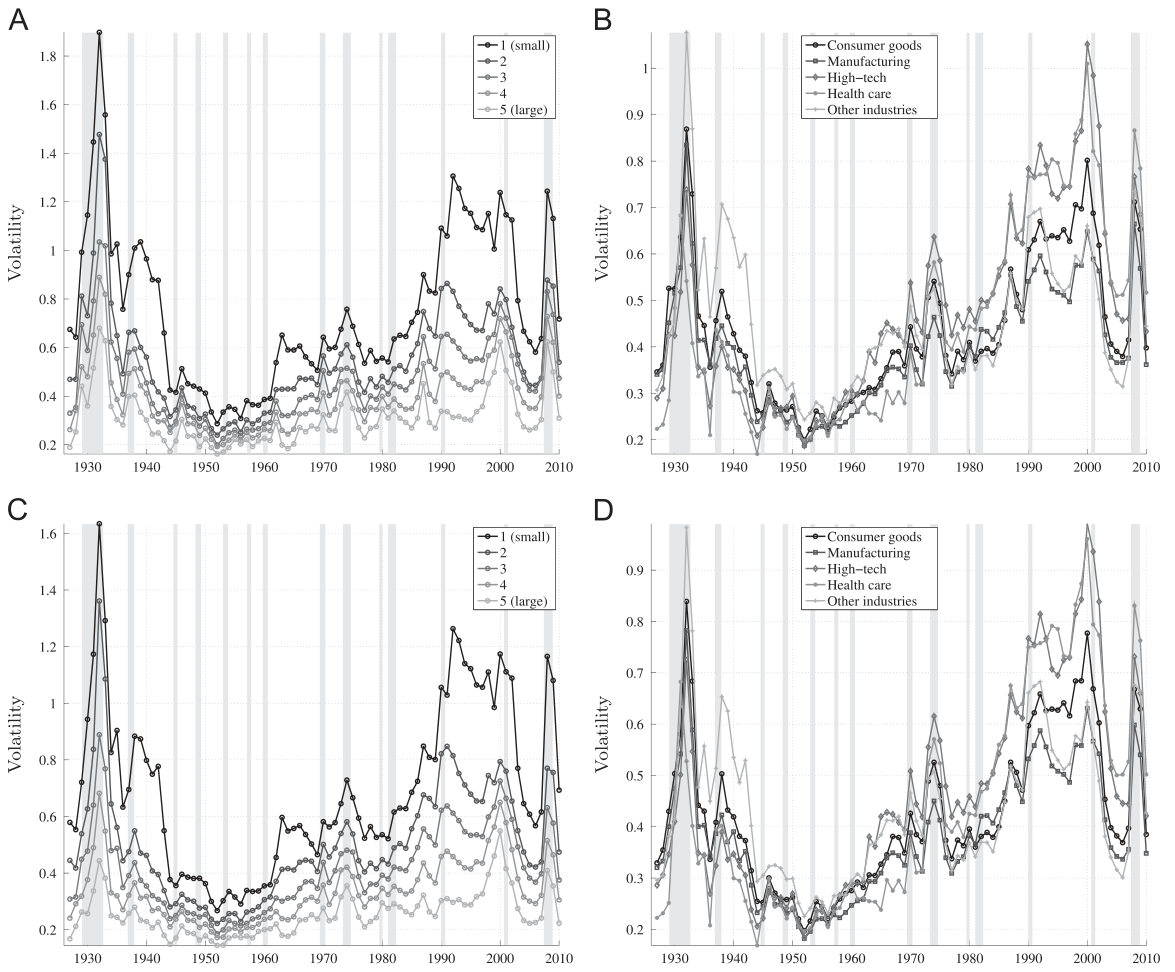
\includegraphics[width=0.7\linewidth]{Files/IV}
		\caption{Total and idiosyncratic return volatility by size and industry group}
	\end{figure}
\end{frame}

\begin{frame}{\href{https://doi.org/10.1016/j.jfineco.2015.09.010}{\textcolor{blue}{Herskovic et al. (2016)}}}
	\begin{figure}
		\centering
		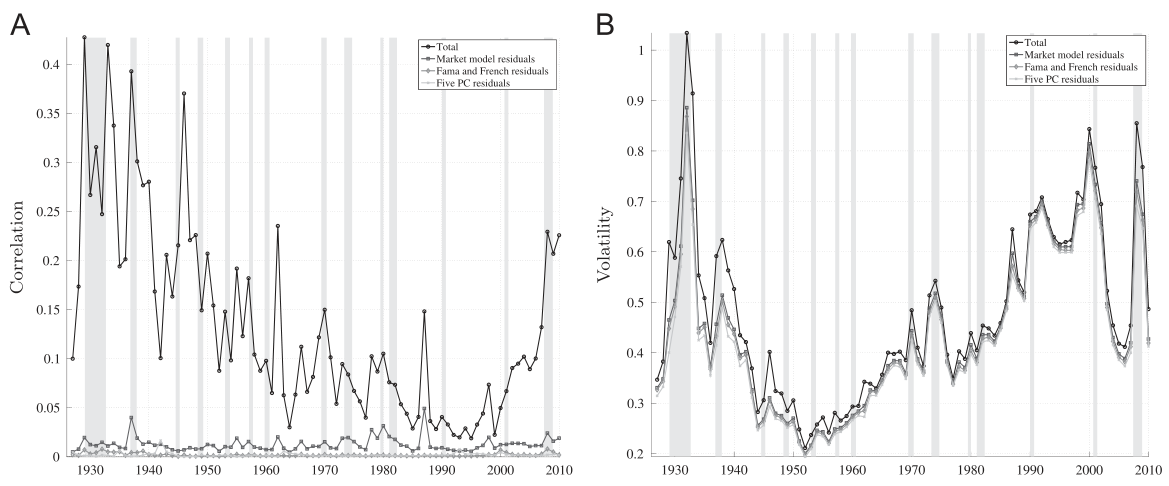
\includegraphics[width=1\linewidth]{Files/IV_vol}
		\caption{Volatility and correlation of return factor model residuals}
	\end{figure}

\end{frame}

\begin{frame}{\href{https://doi.org/10.1016/j.jfineco.2015.09.010}{\textcolor{blue}{Herskovic et al. (2016)}}}
	\begin{figure}
		\centering
		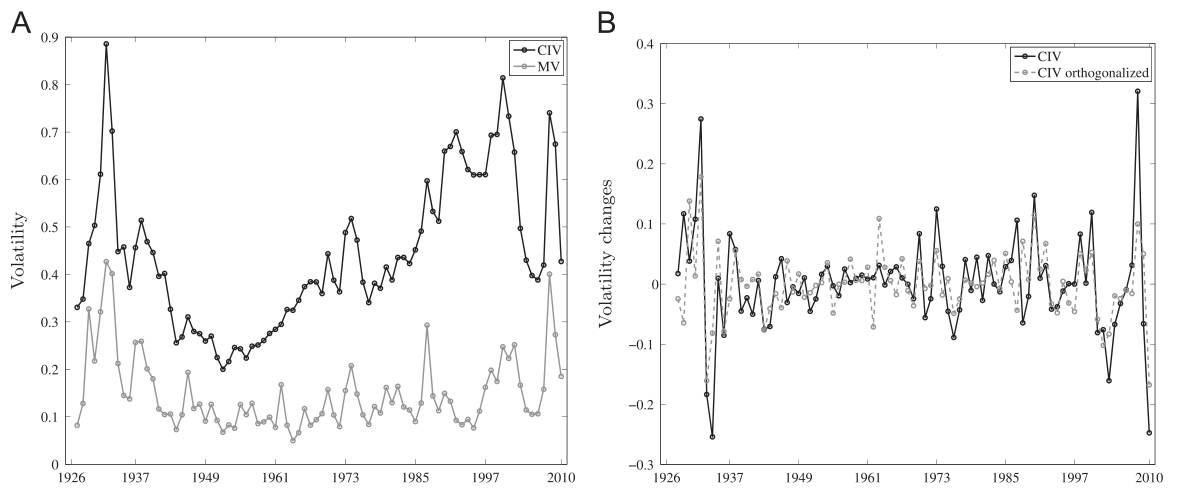
\includegraphics[width=1\linewidth]{Files/IV_shock}
		\caption{Common idiosyncratic volatility (CIV): levels and changes}
		\label{fig:ivshock}
	\end{figure}
\end{frame}

\begin{frame}{\href{https://doi.org/10.1016/j.jfineco.2015.09.010}{\textcolor{blue}{Herskovic et al. (2016)}}}
	\begin{equation}
		r_{i,t} = \alpha + \beta_{\Delta MV_t}  \Delta MV_t + \beta_{\Delta IV_t}  \Delta IV_t
	\end{equation}
\end{frame}

\begin{frame}{\href{https://doi.org/10.1287/mnsc.2018.3036}{\textcolor{blue}{Cooper and Maio (2019)}}}
	\begin{itemize}
		\item \textbf{The ICAPM can be used as a common theoretical background for recent multifactor models.}
		\item The state variables correspond to the rolling sums on the factors. For example, in the case of SMB, the rolling sum is obtained as
		\begin{equation}
			C SMB_{t}=\sum_{s=t-59}^{t} SMB_{s}
		\end{equation}
	\item The first difference in the state variables corresponds
	approximately to the original factors. Thus, this definition tries to resemble the empirical ICAPM literature in
	which the risk factors correspond to autoregressive (orVAR) innovations (or, alternatively, the first difference)in the original state variables.
	\item The state variables can forecast stock market return or stock market volatility.
	\end{itemize}
\end{frame}



\begin{frame}{First Law of Finance}
\begin{itemize}
	\item The consumption-based asset pricing model uses consumption to proxy for \textcolor{red}{$m$}. The CAPM is to use wealth or the rate of return on wealth instead.
	\begin{equation}
		\mathbb{E}_{t}\left[r_{i, t+1}-r_{f, t+1}\right]+\frac{\sigma_{i}^{2}}{2}=-\sigma_{i m}
		\end{equation}
	\item So we prove the return on the stock market or total wealth is linear for $m$. The expected excess market return is a linear function of its own volatility.
	\begin{equation}\label{equ:riskreturn}
		\mathbb{E}_{t}\left[r_{w, t+1}-r_{f, t+1}\right]+\frac{\sigma_{m}^{2}}{2}= \gamma\sigma^2_{m}
		\end{equation}
	\item The equation \textcolor{blue}{(\ref{equ:riskreturn})} is the most commonly used method to test the risk-return trade-off in the empirical research, which is proposed by \href{https://doi.org/10.2307/1913811}{\textcolor{blue}{}Merton (1973)}'s \textbf{intertemporal capital asset pricing model} (ICAPM).
\end{itemize}
\end{frame}

\begin{frame}{Mixed Results}
	But the empirical results are mixed:
	\begin{itemize}
		\item Negative
		\begin{itemize}
			\item \href{https://doi.org/10.1111/j.1540-6261.1993.tb05128.x}{\textcolor{blue}{Glosten, Jagannathan, and Runkle (1993)}}; \href{https://doi.org/10.1111/j.1540-6261.1994.tb05150.x}{\textcolor{blue}{Whitelaw (1994)}}; \\ \href{https://doi.org/10.1111/1540-6261.00555}{\textcolor{blue}{Goyal and Santa‐Clara (2003)}};\href{https://doi.org/10.1016/j.jfineco.2002.06.001}{\textcolor{blue}{Brandt and Kang (2004)}}; \href{https://www.ssrn.com/abstract=4116731}{\textcolor{blue}{Yang (2022)}}
		\end{itemize}
		\item Positive
		\begin{itemize}
			\item \href{https://doi.org/10.1016/j.jfineco.2004.03.008}{\textcolor{blue}{Ghysels, Santa-Clara, and Valkanov (2005)}}; \href{https://doi.org/10.1002/jae.911}{\textcolor{blue}{Bali and Peng (2006)}}; \\
			\href{https://doi.org/10.1111/j.1540-6261.2006.00877.x}{\textcolor{blue}{Guo and Whitelaw (2006)}}; \href{https://doi.org/10.1016/j.jeconom.2015.02.031}{\textcolor{blue}{Bollerslev, Xu, and Zhou (2015)}}
		\end{itemize}
		\item No-correlation
		\begin{itemize}
			\item \href{https://doi.org/10.1016/j.jempfin.2014.06.007}{\textcolor{blue}{Ghysels, Guérin, and Marcellino (2014)}}
		\end{itemize}
	\end{itemize}
\end{frame}

\begin{frame}{Risk-Return Trade Off}
	\begin{itemize}
		\item \textcolor{blue}{This risk-return trade-off is so fundamental in financial economics that it could be described as the ``first fundamental law of finance".}
		\item Do investors really require a positive risk-return trade-off?
		\item Risk-based asset pricing theory does not require the assumption that all investors are always rational and have perfect information.
	\end{itemize}
\end{frame}


\begin{frame}{Empirical Result in China's stock market}
	\begin{itemize}
		\item Stock market excess return: value-weighted stock market return minus risk-free rate
		\item Stock market volatility: stock market realized variance
	\end{itemize}

	Monthly stock market variance is measured as follows:
	\begin{align*}
		%MV_{t} =\sum_{d=1}^{D_{t}}r_{d,t}^{2}+2\sum_{d=2}^{D_{t}}r_{d,t}r_{d-1,t}
		MV_{t} =\sum_{d=1}^{D_{t}}r_{d,t}^{2}
	\end{align*}
	where $ r_{d,t} $ is  the stock market daily excess return in month $t$ on day $d$. $ D_{t} $ is the trading days in month $t$.
\end{frame}



\begin{frame}{Risk Return Trade-Off in China's Stock Market}
	I estimate the OLS regression model as follows:
	\begin{align*}
		r_{t+1} = \alpha + \gamma MV_{t}
	\end{align*}
	The theory implies that the coefficient $\gamma$ should be positively significant.
\end{frame}

\begin{frame}{Empirical Results}
	\begin{table}[!htbp]
		\centering
		\caption{\ \textbf{Risk Return Trade Off}}
		\begin{tabular}{cc}
			\hline
			$ MV $&$ -0.265 $\\
			& $ (-0.555) $\\
			$ adj R^2 $& $ -0.002 $ \\
			\hline
		\end{tabular}
	\end{table}
	The sample spans from 1995 to 2020. The t-statistics are adjusted following Newey and West(1987) for 6-lags.

	\vspace{10pt}
	Question: What's the problem? How to fix it?
\end{frame}

\begin{frame}{1.Conditional Volatility}
	How to measure the conditional volatility?

	\begin{itemize}
		\item Adjust the measurement of volatility
		\begin{itemize}
			\item MV3: \href{https://www.sciencedirect.com/science/article/pii/S0378426624000372}{\textcolor{blue}{Cheng, Guo and Shi (2024)}}
			\item Option implied volatility
		\end{itemize}
		\item Forecast volatility
		\begin{itemize}
			\item OLS: which economic force drive the volatility of stock market?
			\begin{equation}
				MV_t = \beta_1 + \beta_2 * x_{t-1} + \epsilon_{t}
			\end{equation}
			\item GARCH model
			\item Variable selection
			\item Machine learning
			\item Here contains large literature: \href{https://doi.org/10.1016/j.jfineco.2012.06.005}{\textcolor{blue}{Paye (2012)}}
		\end{itemize}
	\end{itemize}
\end{frame}

\begin{frame}{2. Omitted Variable: Hedging Risk}
	\begin{itemize}
	\item \textbf{Note}: How do we link \textcolor{red}{$ m $} to stock market return \textcolor{red}{$r_{w}$} 
	\item Yes, utility function, one-period utility function.
	\item We're interested in determining the exact value of the stochastic discount factor, and we already know that $ m $ is strongly linked to consumption growth. \textbf{The growth of consumption} and \textbf{stock market returns} are a linear relationship when the utility function is \textbf{single period}. What if the utility function \textit{isn't} a single-period utility function?
\end{itemize}
\end{frame}


\begin{frame}{\href{https://www.sciencedirect.com/science/article/pii/S0378426624000372}{\textcolor{blue}{Cheng, Guo and Shi(2024)}}: Conditional Market Variance and Scaled Market Prices}
	\begin{figure}[h]
		{
			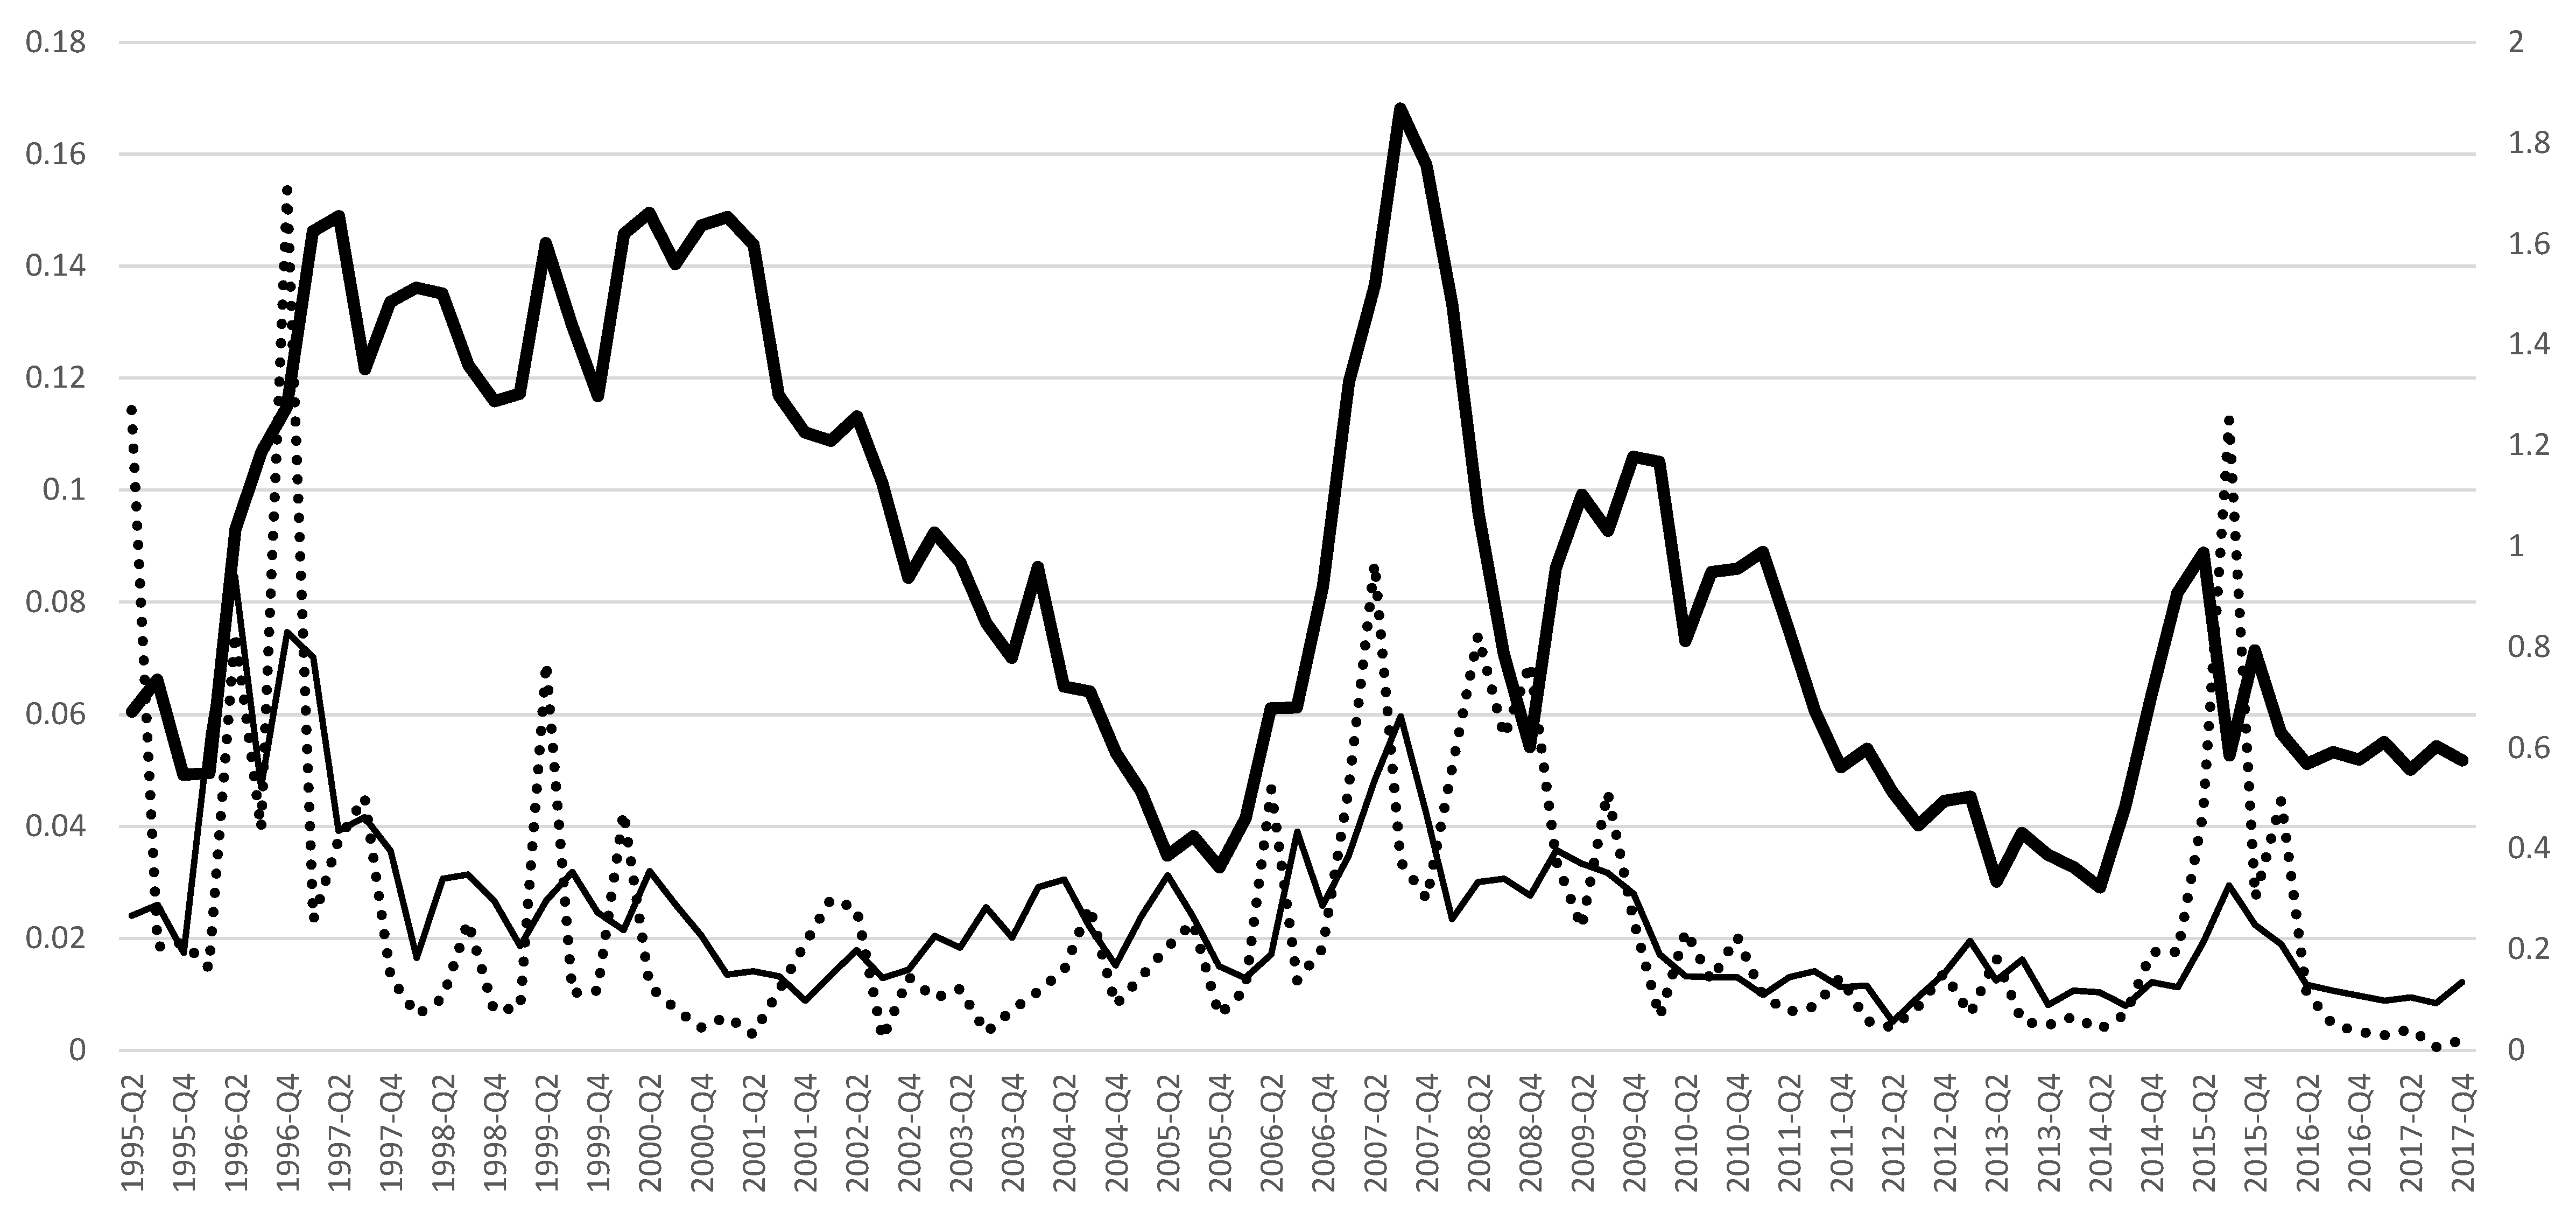
\includegraphics[height=4.5cm, width=10cm]{Files/fig9MVFIT}
		}
		\caption{\ {China's stock market Conditional (Thin Solid Line) and Realized (Dash Line) Market Variance and Market-to-Book Equity Ratio (Thick Solid Line, Right Axis)}} \label{fig:6}
	\end{figure}
\end{frame}


\begin{frame}{\href{https://www.sciencedirect.com/science/article/pii/S0378426624000372}{\textcolor{blue}{Cheng, Guo and Shi(2024)}}: Conditional Market Variance and Scaled Market Prices}
	\begin{figure}[h]
		{
			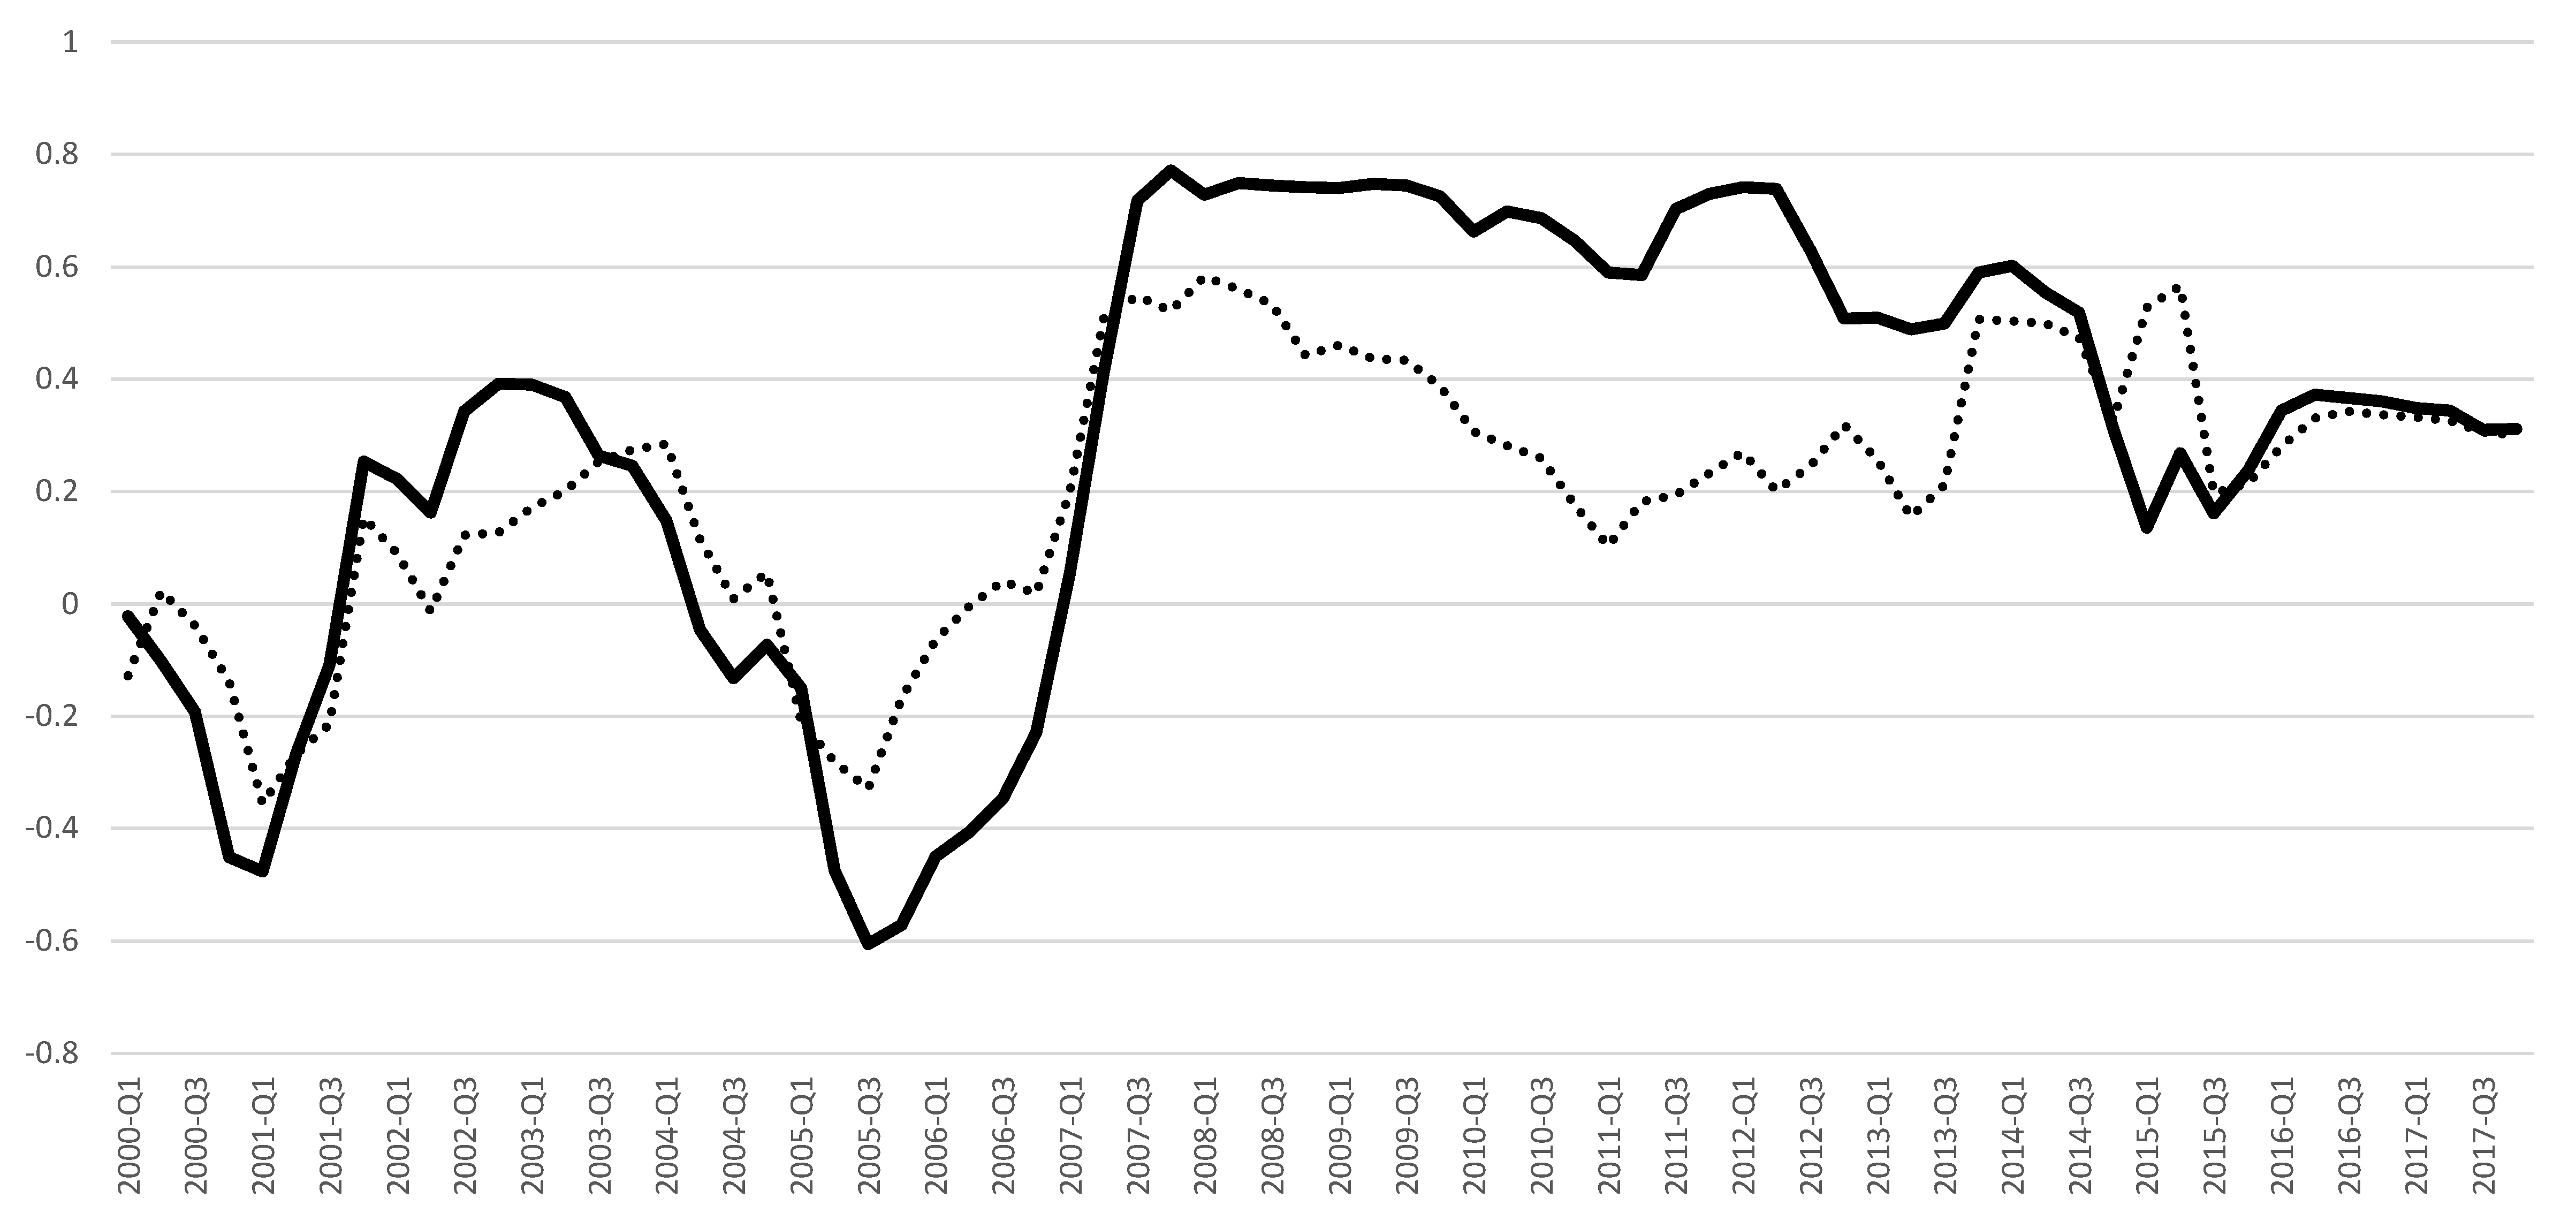
\includegraphics[height=4.5cm, width=10cm]{Files/fig10corr}
		}
		\caption{\ {China's Stock Market Rolling Correlations of Realized (Dashed Line) and Conditional (Solid
				Line) Market Variance with Market-to-Book Equity Ratio}}
	\end{figure}
\end{frame}

\begin{frame}{\href{https://www.sciencedirect.com/science/article/pii/S0378426624000372}{\textcolor{blue}{Cheng, Guo and Shi(2024)}}: Empirical Specifications}

	$MV3_{t}=\omega_{0}+\mathbf{\beta^{\prime}Z_{t-1}}+\zeta_{t}$
	\\
	\vspace{.1in}
	$ERET{t}=\phi+\gamma(\omega_{0}+\mathbf{\beta^{\prime}Z_{t-1}})+\mathbf{\lambda^{\prime}X_{t-1}}+\epsilon_{t}$

	\vspace{.2in}
	Single-factor model
	\begin{itemize}
		\item $\gamma$ is positive
		\item $\lambda$ is zero
		\item Variance and scaled prices have the same forecasting power
	\end{itemize}

	\vspace{.2in}
	Multi-factor model
	\begin{itemize}
		\item $\gamma$ is positive
		\item $\lambda$ is non-zero
		\item Variance and scaled prices have distinct forecasting power
	\end{itemize}

\end{frame}

\begin{frame}{Risk-Return Relation: Quarterly Data}

\begin{table}[ht]
	\small
	\caption{\ \textbf{Market Risk-Return Relationship}}
	\centering
	\label{Table: Risk Return Trade Off}
	\resizebox{110mm}{!}{
		\begin{tabular}{ccccccccccc}
			\toprule
			&$MV3$&$TO$&$ILL\_PS$&$R^2$& $ \gamma $ & $MB$ & $INFL$ & $ERET$  &$R^2$  &OIR(p-value)\\
			\hline \\[-2ex]
			&\multicolumn{4}{c}{$MV3_{t}=\omega_{0}+\mathbf{\beta^{\prime}Z_{t-1}}+\zeta_{t}$}& \multicolumn{5}{c}{$ret_{t}=\phi+\gamma(\omega_{0}+\mathbf{\beta^{\prime}Z_{t-1}})+\mathbf{\lambda^{\prime}X_{t-1}}+\epsilon_{t}$}\\
			
			\cmidrule(r){2-5}  \cmidrule(r){6-10}
			8&0.061&$ \textbf{0.014}^{***} $&$ \textbf{7.789}^{***} $&0.303& $ \textbf{4.489}^{***} $ &  & & & 0.143 & 0.366     \\
			&(0.655)&\textbf{(3.236)}&\textbf{(4.192)}&& \textbf{(3.153)} & &  &  &  &(0.833)   \\

			9&0.039&$ \textbf{0.015}^{***}$&$ \textbf{7.160}^{***}$&0.304  & $ \textbf{5.599}^{***} $ & $ \textbf{-0.128}^{***} $ & &  & 0.217 & 0.098      \\
			&(0.534)&\textbf{(3.894)}&\textbf{(4.131)}&& \textbf{(4.000)} & \textbf{(-3.154)} & &  &  & (0.992)     \\

			10&0.087&$ \textbf{0.013}^{***}$&$ \textbf{7.580}^{***}$&0.301& $ \textbf{5.219}^{***} $ & $ \textbf{-0.135}^{***} $  & &$ \textbf{0.198}^{**} $ & 0.243  & 0.909    \\
			&(1.148)&\textbf{(3.746)}&\textbf{(5.093)}& &  \textbf{(4.319)} & \textbf{(-3.430)}  & &$ \textbf{(2.079)} $ &  & (0.923)   \\

			11&0.056&$ \textbf{0.015}^{***}$&$ \textbf{6.314}^{***}$&0.301& $ \textbf{8.060}^{***}$ & $ \textbf{-0.189}^{***}$ & $ \textbf{-0.675}^{***}$ &  & 0.287 &  2.120   \\
			&(0.913)&$ \textbf{(4.133)} $&$ \textbf{(4.277)} $&& $ \textbf{(4.693)} $ &$ \textbf{(-4.690)} $  & $ \textbf{(-4.708)} $ &  &   & (0.714) \\

			12&0.095&$ \textbf{0.013}^{***}$&$ \textbf{6.505}^{***}$& 0.300 & $ \textbf{7.751}^{***}$ & $ \textbf{-0.181}^{***}$ & $ \textbf{-0.627}^{***}$ & 0.129 & 0.306 &  3.194   \\
			&(1.472)&$ \textbf{(3.990)} $&$ \textbf{(5.347)} $& & $ \textbf{(5.009)} $ & $ \textbf{(-4.677)} $ & $ \textbf{(-5.072)} $ & (1.425) &   & (0.670)  \\

			\bottomrule
			\vspace{1pt}
	\end{tabular}}
\end{table}
\end{frame}

\begin{frame}{Risk-Return Relation: Alternative Measures}

	\begin{table}[ht]
		\caption{\textbf{Alternative Scaled Market Price Measures}}
		\label{Table A3}
		\centering
		\resizebox{110mm}{!}{
			\begin{tabular}{ccccccccc}
				\toprule
				%\multicolumn{9}{l}{Panel A: Market Variance}\\
				%\hline \\[-2ex]
				& $\gamma$&$ MB $&$ PD $&$ PE $&$ PS $&$ PC1 $&$ R^2 $&OIR(p-value)\\
				\hline \\[-2ex]
				1&$ \textbf{5.599}^{***} $ &$ \textbf{-0.128}^{***} $&&&&&0.217&0.098\\
				&\textbf{(4.000)} &\textbf{(-3.154)}&&&&&&(0.992)\\
				%\hline \\[-2ex]
				2&$ \textbf{5.671}^{***} $ &&$ \textbf{-0.080}^{***} $&&&&0.202&0.435\\
				&\textbf{(4.058)} &&\textbf{(-2.836)}&&&&&(0.933)\\
				%\hline \\[-2ex]
				3&$ \textbf{5.983}^{***} $ &&&$ \textbf{-0.093}^{***} $&&&0.187&1.961\\
				&\textbf{(3.964)} &&&\textbf{(-2.890)}&&&&(0.581)\\
				%\hline \\[-2ex]
				4&$ \textbf{5.594}^{***} $ &&&&$ \textbf{-0.082}^{**} $&&0.197&0.595\\
				&\textbf{(3.680)} &&&&\textbf{(-2.539)}&&&(0.898)\\
				%\hline \\[-2ex]
				5&$ \textbf{5.782}^{***} $ &&&&&$ \textbf{-0.026}^{***} $&0.204&0.514\\
				&\textbf{(3.965)} &&&&&\textbf{(-2.930)}&&(0.916)\\
				\bottomrule
				\vspace{1pt}
		\end{tabular}}
	\end{table}
\end{frame}




\end{document}
